\documentclass[a4paper,11pt]{article}

\title{Exercize on unfolding distributions}
\author{ACM}
\date{\today}

%%
\usepackage{bbding}
\usepackage{ifthen}
\usepackage{graphicx}
\usepackage{amsmath}
%
\setlength{\parindent}{0pt}

\newcommand{\difficulty}[1]
                {
                \vspace{-30pt}
                \begin{flushright}
                \mbox{
                \ifthenelse{ #1 = 1 }{\FiveStar \FiveStarOpen \FiveStarOpen \FiveStarOpen \FiveStarOpen} {}
                \ifthenelse{ #1 = 2 }{\FiveStar \FiveStar \FiveStarOpen \FiveStarOpen \FiveStarOpen} {}
                \ifthenelse{ #1 = 3 }{\FiveStar \FiveStar \FiveStar \FiveStarOpen \FiveStarOpen} {}
                \ifthenelse{ #1 = 4 }{\FiveStar \FiveStar \FiveStar \FiveStar \FiveStarOpen} {}
                \ifthenelse{ #1 = 5 }{\FiveStar \FiveStar \FiveStar \FiveStar \FiveStar} {}
                }
                \end{flushright}
                }




\usepackage[english]{babel}
%FloatBarrier
\usepackage{placeins}
%H
\usepackage{float}
\usepackage{amsmath,amssymb,amsfonts}
\usepackage{graphicx}
\usepackage{amsmath}
\usepackage[pdftex,hyperfootnotes=false,pdfpagelabels,pagebackref]{hyperref}

% to make a analitical index/glossaries
%\usepackage[acronym,xindy,nonumberlist]{glossaries}
\usepackage[acronym,nonumberlist]{glossaries}
%\usepackage{makeidx}
\makeglossaries
%\makeindex

\usepackage{booktabs}

%caption
%\usepackage[font=small,format=plain,labelfont=bf,margin=0.05\columnwidth]{caption}
\usepackage[font=small,format=plain,labelfont=bf,margin=0.05\columnwidth]{caption}


%%%% DEFINE COMMANDS %%%%%%%%%%%
\newcommand{\meas} {\ensuremath \vec{y}}
\newcommand{\truth}{\ensuremath \vec{x}_\textup{T}}
\newcommand{\resp} {\ensuremath \mathbf{R}}
\newcommand{\back} {\ensuremath \vec{b}}

\newcommand{\respt}{\ensuremath \mathbf{\tilde{R}}}
\newcommand{\strength}{\ensuremath \vec{\mu} } 

\newcommand{\mc}{\ensuremath \vec{x}_\textup{MC}}
%% I version
\newcommand{\truthI}[1]{\ensuremath x^\textup{T}_{#1}}
\newcommand{\strengthI}[1]{\ensuremath \mu_{#1} }
\newcommand{\mcI}[1]{\ensuremath x^\textup{MC}_{#1}}
\newcommand{\respI}[2]{\ensuremath R_{#1,#2} }
\newcommand{\resptI}[2]{\ensuremath \tilde{R}_{#1,#2} }

%% FIG 
\newcommand{\Left}{\mbox{(Left)}}
\newcommand{\Right}{\mbox{(Right)}}

%%%  Draft
\newcommand{\fixme}[1]{ \mbox{\bf{FIXME:} \it{#1}} } 


\newacronym{MC}{MC}{Monte Carlo}
\newacronym{BLUE}{BLUE}{best linear unbiased estimator}
\newacronym{ML}{ML}{maximum likelihood}
\newacronym{SVD}{SVD}{singular value decomposition}




\begin{document}
\maketitle

\section{Introduction}
Unfolding is the ``art'' of being able to undo detector effects, such as smearings, efficiencies or background contaminations.
Unfolding techniques refers to a set of statistical tools explained in many books such as Ref.~\cite{Cowan}, 
or summurized in short letter and articles \cite{Cowan:unfolding}. 
Different software suites provede an implementation of such methods; 
in particle physics one of the most spread is {\scshape RooUnfold} \cite{RooUnfold}, 
which can be used within the {\scshape root} software \cite{ROOT}. 

The basic idea behind unfolding is the fact that (at least on certain observables) detector acts linearly on the shapes; this is the case for example for cross-section measurements, where the observables is the total number of event registered in the detector.
The equation we will encounter is the following:
\begin{equation}
	\meas= \respt \cdot \truth + \back
	\label{eqn:base}
\end{equation}
it means that the measured spectra ($\meas$) can be obtained by a smearing and efficiency ($\respt$) applied on the truth distribution ($\truth$). To that a possible background ($\back$) can be added to the measured distribution; this background can come from different sources, like different processes, but also different region of the phase-space where the smearings effects can lead to migration inside the region of interest.

Equation~\ref{eqn:base} can come in different shapes, one of the most relevant is the rescaling of it with respect to a particular truth/prediction \cite{SVD}:
\begin{equation}
	\meas = \resp \cdot \strength + \back
\end{equation}
where $\strengthI{i} = \frac{\truthI{i}}{\mcI{i}} $ and  $\respI{i}{j} = \resptI{i}{j} \cdot \mcI{i} $, making the content of the response matrix $\resp$ the actual number of expected events.

\subsection{Code and Software}
In HEP the most widespread code is {\scshape root} (and {PyRoot}) with the additional package of {\scshape RooUnfold}.

\section{Understanding unfolding}
\difficulty{2}

The first point of understand how unfolding operate is to deal with the smearing of the distribution.
Suppose to have a fully efficient detector that has just a poor gaussian resolution of $0.4 a.u.$, as given in the attachments:
\begin{enumerate}
	\item Write the inversion method to unfold the distribution without random fluctuations
	\item Use the inversion method to unfold the distirbution with random fluctuations in the attachment; these are obtained with a gaussian smearing of $1.0$ event.
	\item discuss the result.
\end{enumerate}
\begin{figure}[H]
	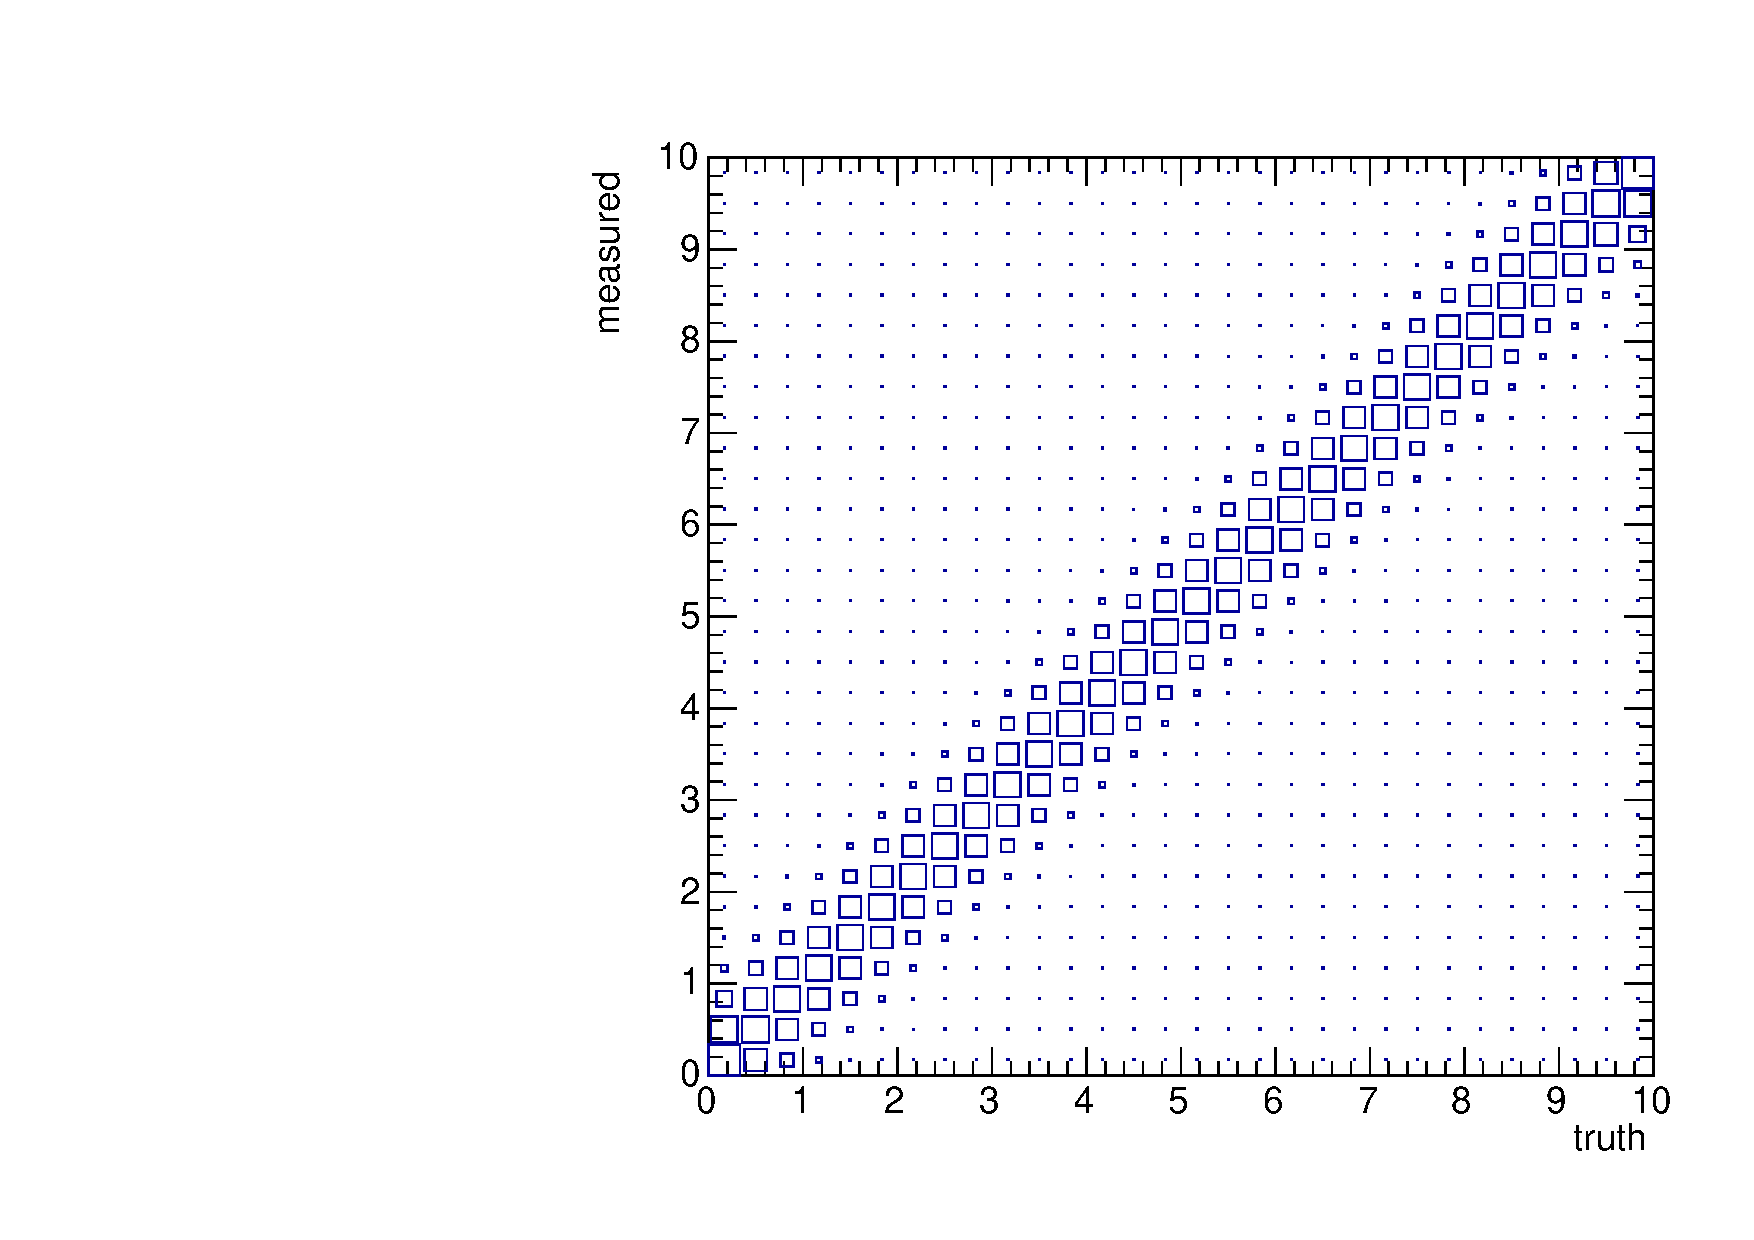
\includegraphics[width=0.49\textwidth]{figs/respt.pdf}
	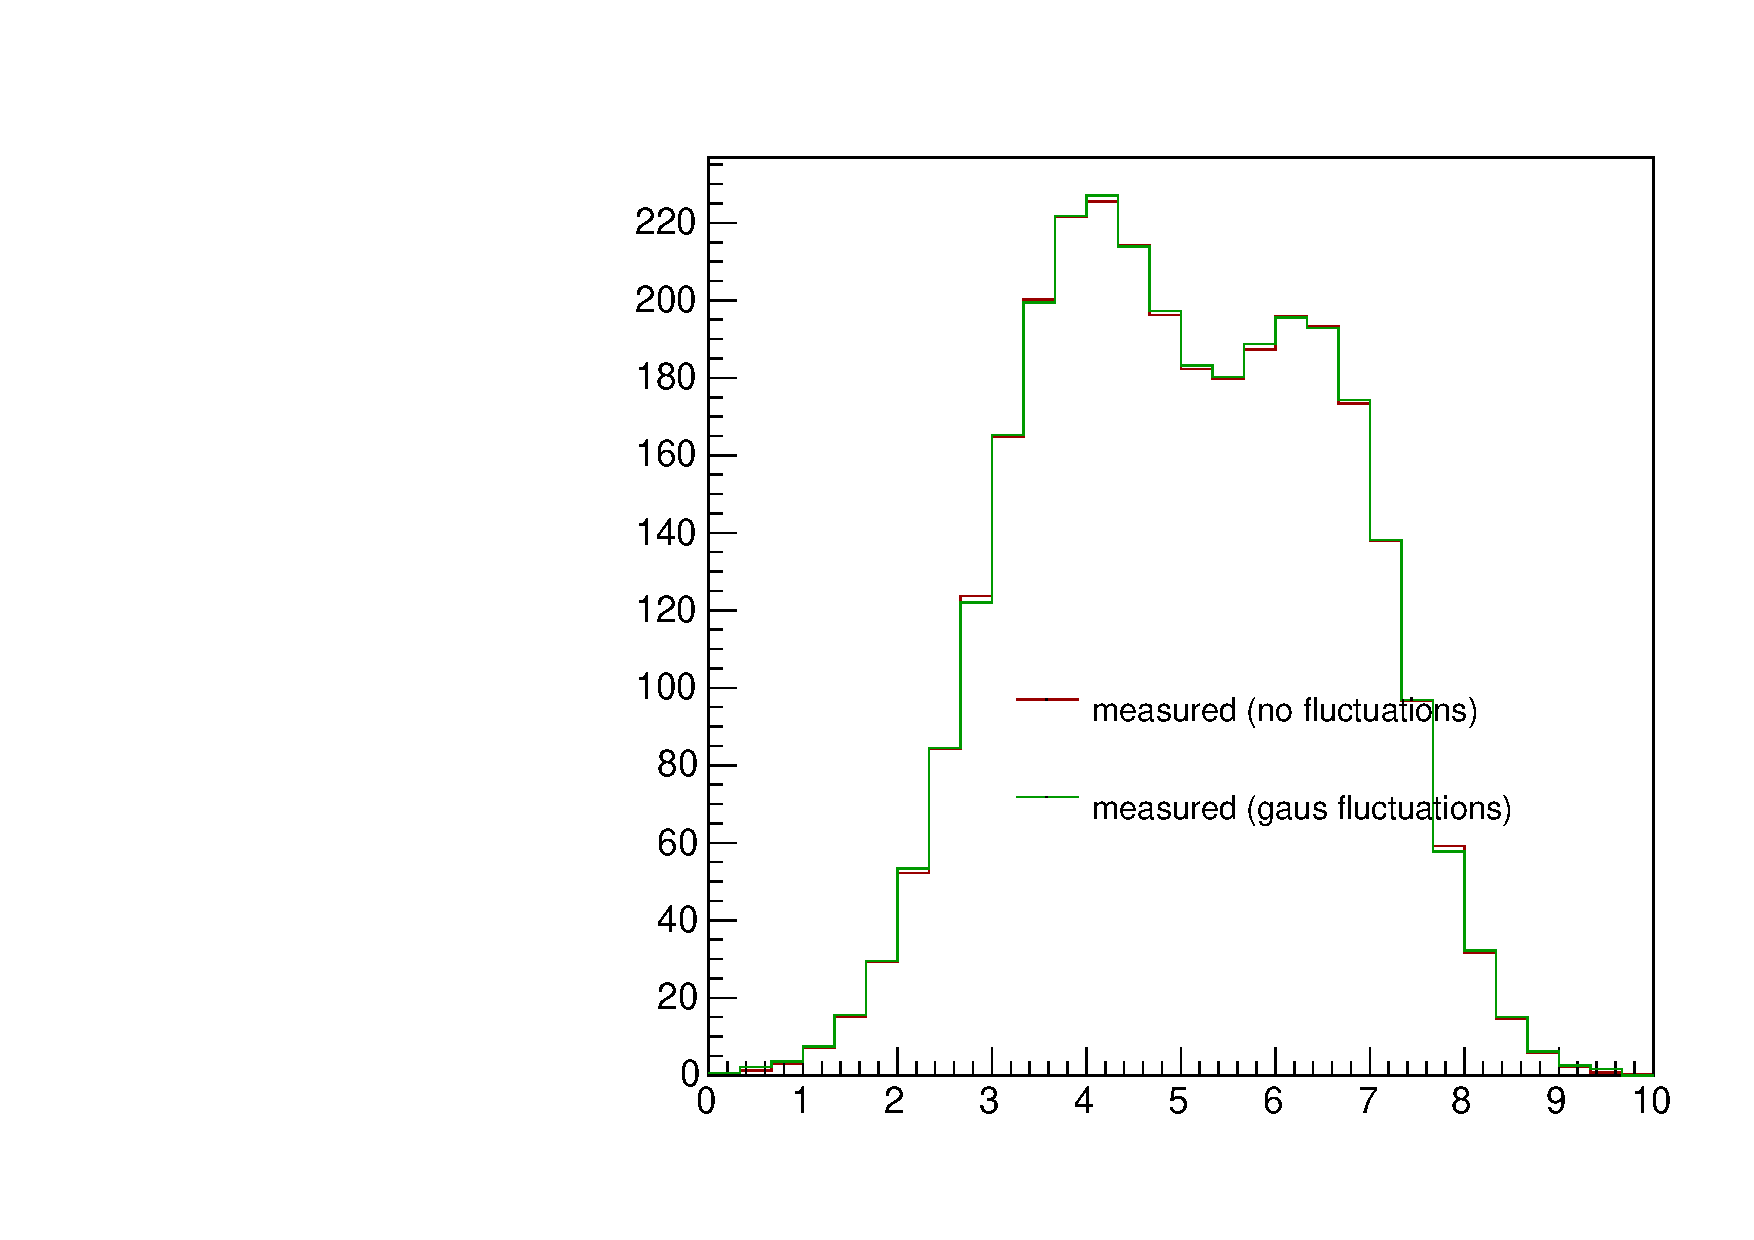
\includegraphics[width=0.49\textwidth]{figs/reco.pdf}
	\caption{
		\label{fig:exe1}
		Left: smearing matrix ($\respt$) 
		Right: reconstructed distributions with and without random fluctuations.
	}	
\end{figure}
\FloatBarrier

\section{Regularization}
\difficulty{3}

The most used regularization methods are the iterative-method based on the Bayes' theorem \cite{dAgostini} and the Tickonov regularization, which is implemented efficiently with the \gls{SVD} decomposition \cite{SVD}.
Using the histogram with fluctuations of the exercize above:
\begin{enumerate}
	\item provide an unfolded distribution with the different regularization parameters.
	\item discuss the effect and the limits of the regularization parameter in the two methods.
	\item discuss how you would choose the regularization parameter.
\end{enumerate}

\section{Constructing a Response Matrix}
\difficulty{4}

What it usually happens is that response matrixes are built from event-based \gls{MC} simulation.
In this section you are asked to unfold a given distribution, constructing before the response matrix.

Event-based \gls{MC} simulations, 
if produced with different luminosity than the one delivered by the machine, needs to be reweighted 
in order to have the correct \emph{cross-section} and \emph{luminosity} of the data we are comparing to,
Moreover, it is common practice to increase the number of event produced in the \gls{MC} simulation in ``interesting'' 
region of the phase space, therefore these weights cannot be assumed uniform.

Unfortunately, the \gls{MC} simulation is not-perfect and needs to be corrected for small effects.
Typically these are small scale-factors measured with techinques like the \emph{tag-and-probe}. 
This type of weights are aimed to correct the difference in efficiency observed in the different objects 
and are assumed to be uncorrelated.


%%%%%%%%%%%%%%%%%%%% BIBLIO %%%%%%%%%%%%%%%%%%%%%%
\FloatBarrier
\nocite{*}
%\bibliographystyle{acm}
\bibliographystyle{acmunsrt}
%\addcontentsline{toc}{section}{\refname}
\bibliography{UnfoldingExe}
%%%%%%%%%%%%%%%%%%
\cleardoublepage

\end{document}
